%%This is a very basic article template.
%%There is just one section and two subsections.
\documentclass{article}
\usepackage{appendix}
\usepackage{amsmath}
\usepackage{caption}
\usepackage{placeins}
\usepackage{graphicx}
\usepackage{subcaption}
\usepackage{longtable}
\usepackage{tikz}
%\usepackage[active,tightpage]{preview}
\usepackage{natbib}
\bibpunct{(}{)}{,}{a}{}{;} 
\usepackage{url}
\usepackage{nth}
\usepackage{authblk}
% for the d in integrals
\newcommand{\dd}{\; \mathrm{d}}
\newcommand{\tc}{\quad\quad\text{,}}
\newcommand{\tp}{\quad\quad\text{.}}

% working on this need to concatenate file name based on sex and variable name
\newcommand\Cell[1]{{\raisebox{-0.05in}{\includegraphics[height=.2in,width=.2in]{Figures/ColorCodes/\expandafter#1}}}}  

\defcitealias{HMD}{HMD}

\begin{document}

\title{Time-to-death patterns in markers of age and dependency}

\author[1]{Tim Riffe\thanks{triffe@demog.berkeley.edu}}
\author[1]{Pil H. Chung}
\author[2,3]{Jeroen Spijker}
\author[4]{John MacInnes}
\affil[1]{Department of Demography, University of California, Berkeley}
\affil[2]{Department of Geography, Universitat Aut{\`o}noma de Barcelona}
\affil[3]{Vienna Institute of Demography}
\affil[4]{School of Social and Political Science, University of Edinburgh}

\maketitle

\begin{abstract}
We aim to determine the extent to which variables commonly
used to describe health, well-being, and disability in old-age vary primarily
as a function of years lived (age), years left, or as a function of both. We analyze data from the US Health and Retirement Study to estimate
chronological age and time-to-death patterns in 60 such variables. We describe
results for individuals with 15 or fewer remaining years of life, after age 70
and whose completed lifespans do not exceed 100. Our results show that most
markers used to study well-being in old-age vary along both time dimensions, but
that variation over remaining years of life is typically much stronger for
the age-ranges and variables examined.
\end{abstract}

\section*{Background}

For an
individual, age across the lifecourse is comprised two components: time since
birth and time to death, the chronological and thanatalogical dimensions of
age, respectively. In the aggregate, thanatological age is determined
by the mortality rate schedule to which a birth cohort is subject until its
extinction. Individuals do not know their thanatological age with certainty. To
overcome this we project an expectation of lifespan, based on scenarios or extrapolations of how mortality
rates might change over time. Prospectively, decreasing mortality has the effect
of moving population into higher thanatological ages, thereby increasing
remaining life expectancy \citep{sanderson2005average}. In this case,
the notion and measure of future remaining lifespan is elastic, subject to uncertainty.
In retrospect (after the death of a cohort), the thanatological age structure of
a population is a fixed characteristic. Furthermore, since a closed birth cohort
is akin to a stationary population,\footnote{The age structure of a birth cohort over time is proportional to the $l(x)$ column of the lifetable that describes its
mortality, which is proportional to the stable age structure determined by
the Lotka-Euler renewal model when the intrinsic growth rate is equal to zero.}
the chronological and thanatological age profiles are identical
\citep{brouard1989mouvements,vaupel2009life,rao2014generalization}. Yet, even in
the symmetrical case of stationary populations, the age profiles of other
demographic characteristics in the population are decidedly not symmetrical when
viewed chronologically or thanatologically. Distinct patterns emerge in the
aggregate due to an interaction between lifespan variation and the age profile(s) of
demographic characteristics.\footnote{To state that a characteristic is a function of either
age perspective does not imply that age causes the given characteristic to vary,
but rather that a characteristic varies in some smooth, regular, or parsimonious
way over age.}

Some life
transitions, states, and state intensities are almost exclusively a function of
time to death. In cases where a characteristic strongly varies as a function of
time to death (e.g., increases exponentially with the approach to death),
the common practice of aggregation over chronological age may misrepresent time
trends and misguide analyses about change over time and expectations for the
future. Retrospective measurment of thanatological age is useful in such
cases, as a way of separating trends in characteristics with time-to-death
patterns from trends in mortality. This step lends clarity to the understanding
of how characteristics vary over the lifespan and over time.

This perspective is especially important when assessing the impact of
``population ageing''.
To the extent that the health, welfare, and social care demands of a
population are functions of thanatological rather than chronological age
structure, forecasts of the social and economic ``costs'' of ageing that are
based only on chronological age profiles are vulnerable to being seriously
misleading.
In our concluding discussion we return to this point.

Work has been done on this topic in other domains, and
topics examined can be roughly categorized into two types: 1) things that are a
function of apparent or perceived time to death
\citep{hamermesh1985expectations,hurd1995evaluation,carstensen2006influence,gan2004subjective,biro2010subjective,salm2010subjective,van2010living,cocco2012longevity,payne2013life,balia2013survival},
and 2) things that are a function of actual time to death
\citep{miller2001increasing,seshamani2004longitudinal,werblow2007population}.
The former are mostly studies on cognitive transitions and economic or
health behaviors, while the latter are mostly studies on health expenditure.
Another branch of research relates perceived and actual remaining lifetime
\citep{perozek2008using,delavande2011differential,post2012longevity,kutlu2013individuals}.
In this paper we will expand the second group, focusing on a broad range of
questions from the US Health and Retirement Study \citep{HRS}.

Data classified by chronological age, like census population counts, can be
transformed into thanatological age using some simple lifetable
assumptions\footnote{A paper on this topic is currently under review \citep{riffe2014paaposter}. \citet{brouard1986structure,
brouard1989mouvements} had already done the same thing some 30 years earlier, and we understand that
S. Scherbov also unwittingly produced the same result over a decade ago. It is
safe to say that most demographers are still unaware of the method, however.}.
This transformation yields the thanatological age structure of the population
under a particular set of mortality assumptions.
However, such lifetable-based transformations are idealized, and in many informal
conversations the question has been raised as to which life transitions
may actually be better understood as a function of thanatological
age rather than chronological age.

The present study is exploratory. We have the impression
that such patterns are mostly novel to demographers and as-yet unincorporated in
population-level indicators of ageing or disability. We aim to identify a
range of domains in which it makes sense to think from a
thanatological perspective. 

In the following sections we describe our
approach to this exercise. In short, for a given characteristic, we produce a
demographic surface, where chronological age and thanatological age are the
primary x and y axes, respectively.
We then characterize this surface in a simple way by determining the average direction of steepest ascent on the surface,
which tells us the primary direction of variation. If something varies more along the thanatological axis, then we call it a thanatological characteristic, if it varies more along the chronological axis, we call it a chronological characteristic. We then derive the degree to which a characteristic is thanatological as a percentage.

\section*{Data \& Method}
All findings reported in this paper are based on data from the US Health and
Retirement Study (HRS). We use the Rand edition of the data, which is
conveniently merged across all ten waves, and we calculate thanatological age
based on date of death information in the mortality followup module. We
restrict the sample to only those individuals that have died, which reduces the
dataset from 36986 individuals with an average of 5 interviews each to 11947
deceased individuals with an average of 4.25 interviews each. Further winowing
from our weighting criterion reduces the dataset to
11520 individuals with 4.1 interviews each on average. Person-weighting is
described in the following section. In the present exploration, we do not examine
within-individual variation, and each instance of an interview is treated as an
independent observation.

\subsection{Weighting}
Person weights
are needed in order to estimate population-level means.
One difficulty with the HRS is that the institutionalized population is treated
as a second target population. In all waves but 5 and 6, there are no person weights
assigned to institutionalized individuals. In some cases we try to fill the gap according to some simple
assumptions. If the individual was assigned a weight in a previous wave, we
carry this weight over as a constant, unless there was also a non-zero weight in a future interview, in
which case we assign the weight according to the within-individual linear
pattern. Some individuals are in the dataset, but are
excluded (spouses mostly) for not having reached age 61. In these
cases, we discard interviews with no person weights at young ages. 

\subsection{Age}
Thanatological age is calculated for each individual as the lag between
interview and death dates expressed as decimal years. Chronological age is
calculated as the lag between birth and interview date in decimal years. Birth
dates and death dates in the original data are typically rounded up to the end
of the month, but this is more than enough precision for our purposes. Since we
are interested in comparing characteristics over both chronological age and
thanatological age simultaneously, we are interested in having estimates over a
good spread of both age perspectives.
Figure~\ref{fig:counts} shows the case count in two-year age groups over the
range of ages that are in the data and included for this study (yellow bin).
Darker blues indicate higher case counts, and the contours approximate counts at
this level of aggregation. In practice, these counts are a maximum, since
particular variables studided may be missing.

\begin{figure}[!h]
\centering
\caption{Case counts in two-year age bins. Chronological age (Years lived) on
the x axis and thanatological age (Years lives) on the y axis. Darker blues
indicate higher case counts.}
\label{fig:counts}
\begin{subfigure}{\linewidth}
	\caption{Males}
	\vspace{-1em}
	\label{fig:MalesCases}
	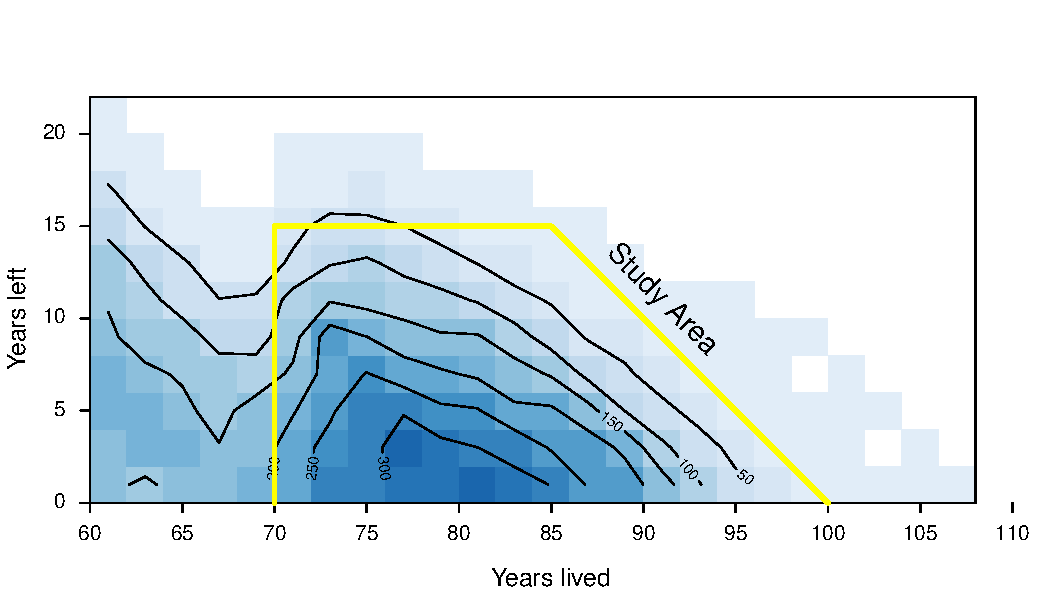
\includegraphics[scale=.7]{Figures/CaseCountMales.pdf}
\end{subfigure}
\\
\begin{subfigure}{\linewidth}
    \caption{Females}
   \vspace{-1em}
	\label{fig:FemalesCases}
    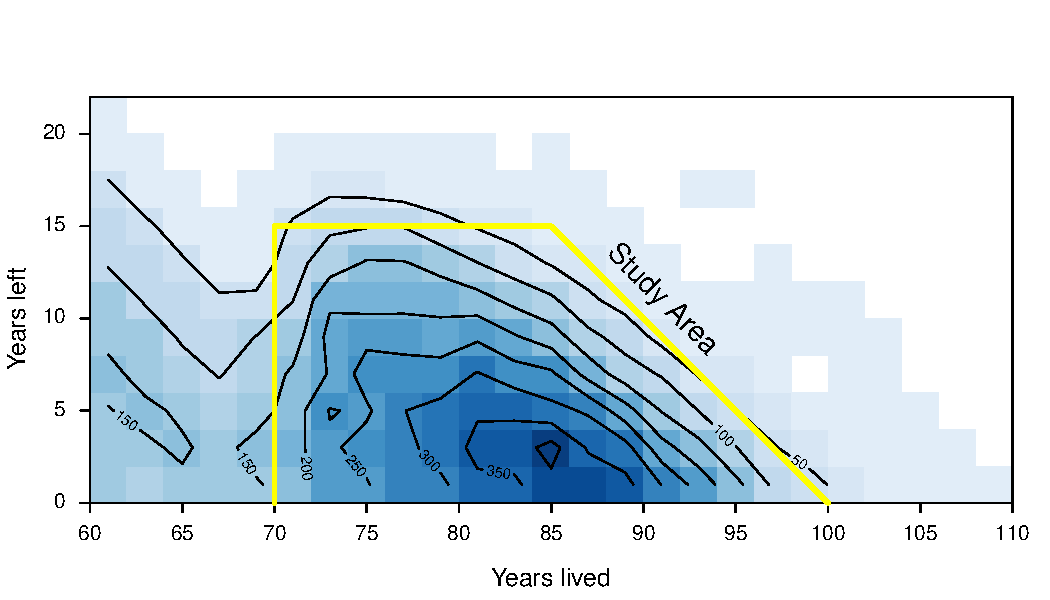
\includegraphics[scale=.7]{Figures/CaseCountFemales.pdf}
\end{subfigure}
\end{figure}

Note that Figure~\ref{fig:counts} resembles a Lexis surface in some ways, but it
is not organized by years or birth cohorts. Instead, years and birth cohorts in
the data are overlapped and treated as a single period and a single birth
cohort. We limit the study area to chronological ages 70 and higher, and
thanatological ages 15 and lower, such that the sum of the two ages does not
exceed 100. These bounds allow for reasonably stable estimates of surfaces for
the studied characteristics. We cut off below chronological age 70 in order to
remove some patterns that appear to be due to retirement rather than
senescence processes, and also to avoid some potential compositional bias, as
these are the typical ages of recruitment for the HRS.\footnote{Conceivably, the study
area could be expanded after the addition of future mortality follow-ups.} 

\subsection{Variables}
We aim for a broad overview of the age variation across different dimensions of
old-age disability and well-being. For this reason we select a wide variety of
questions from the HRS data to describe here. These include questions
grouped roughly into the following categories: Activities of daily living (ADL),
instrumental activities of daily living (IADL), measures of healthcare utilization, functional and chronic conditions, psychological
measures, and health behaviors. In all, we report summary results from 60
individual items.

We judge the degree of chronological versus thanatological age variation by
creating surfaces over both age dimensions, and for this each survey question
was required in a format suitable for numeric operations. This requires some
compromises in data quality, since some coded responses are less directly
quantifiable, and our conversions were at times ad-hoc. The treatment of
individual variables will be described in an appendix in a future
revision of this paper.

\subsection{Loess smoothing}
Direct tabulations of the weighted data are possible, and usually not too noisy,
but surface legibility is enhanced by estimating based on a loess-smoothed
surface. For each variable of interest, we convert values to a numeric scale.
For variables where a numeric scale is not the natural form of observation, we
describe the conversion protocol in an appendix\footnote{Variable appendix not
included in proposal.}. We then fit a two-dimensional loess model\footnote{We
fit using the \texttt{loess()} function in base \texttt{R}
\citep{cleveland1992local,Rcore2013} and its related prediction method. The
smoothing parameter, \texttt{spar}, is set to 0.5.} to the weighted
individual-level data for each sex separately, where the numeric characteristic value is the dependant variable and individual decimal values of thanatological and chronological age are the independent variables.
Weighting is then explicit by person-weights, and implicit by point density
within the surface. All individuals are included in the model fit, but point
predictions are calculated for a grid of single thanatological and chronological
ages within the study area outlined in Figure~\ref{fig:counts} and described in
the previous section. 

\subsection{Finding the fall-line}
The model fit for each variable is used to produce a contour surface, which can
be interpreted visually. In most situations it is obvious to the eye whether a
variable operates over thanatological age or over chronological age, but there
are also some instances where both are at play, the pattern is evidently
distorted by underlying cohort heterogeneity, or where the relationship is
unclear. An example surface for self-reported health (SRH) is shown in
Figure~\ref{fig:srh}.

\begin{figure}[!h]
    \centering
    \caption{Mean male SRH by years lived (x axis) and years left (y axis).}
    \label{fig:srh}
	\vspace{-2em}
	\makebox[\textwidth][c]{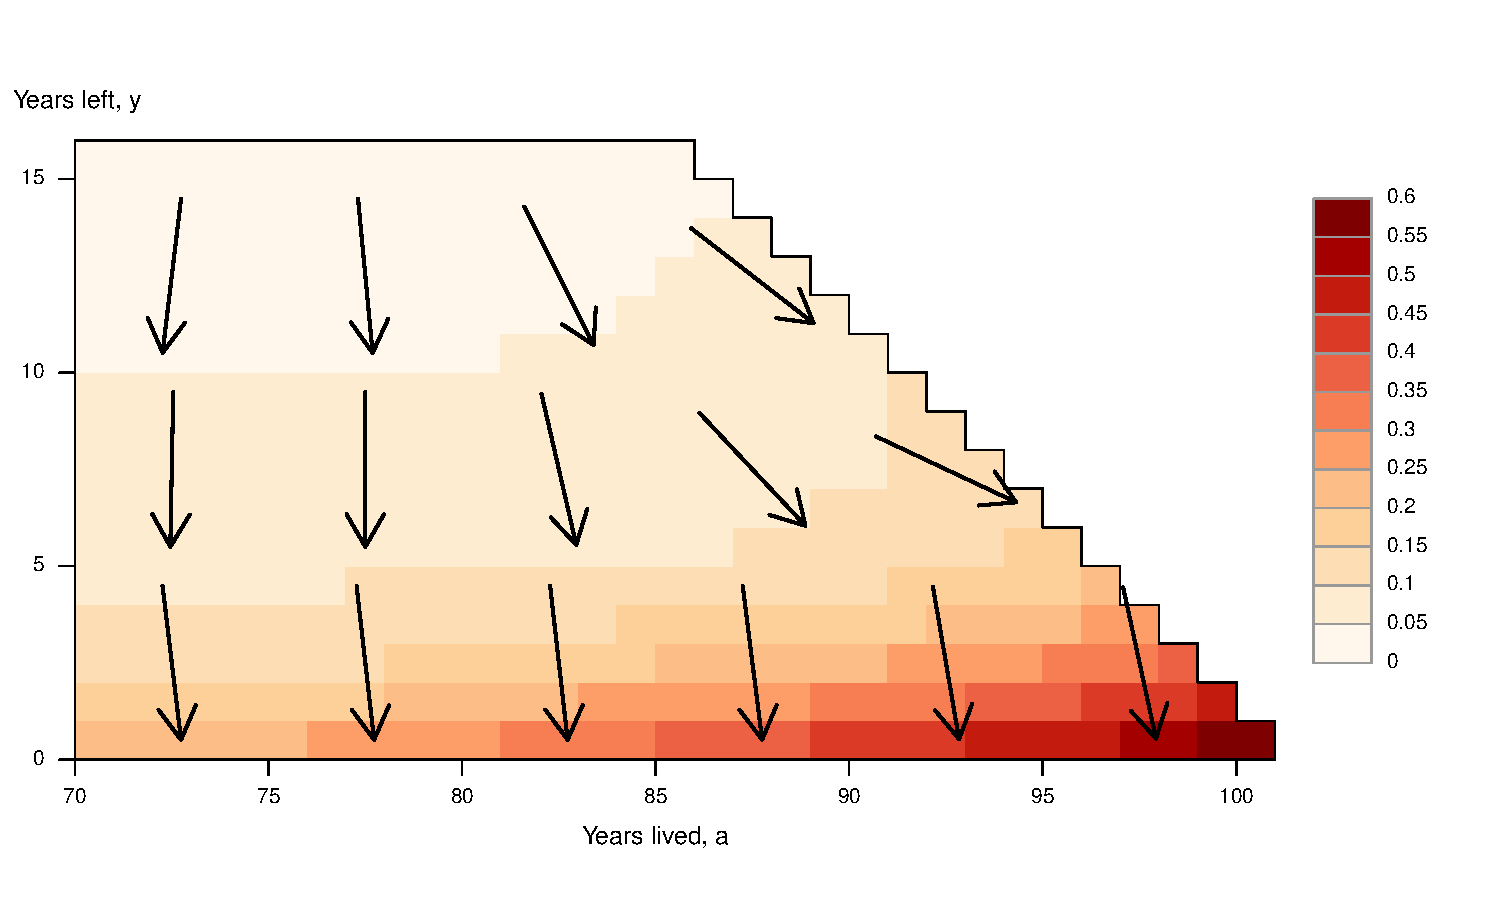
\includegraphics[scale=.6]{Figures/SurfExampleMalesSRH.pdf}}
\end{figure}

In the case of Figure~\ref{fig:srh} note that there is regular variation in the
direction of both axes, but that the variation over thanatological age (y axis)
is sharper, i.e., it implies a steeper climb than does the apparent decrease
over chronological age. 

In order to characterize this surface, we find the direction
of steepest ascent for a regular grid of points. These directions are shown with
arrows in Figure~\ref{fig:srh}. If the direction is exactly $90^\circ$ or $270^\circ$,
then we know that the process is essentially a thanatological one, at least in
the age-range studied. If the direction is $0^\circ$ or $180^\circ$, then the
characteristic can be said to be chronological. In our experience, most
variables that we might be interested in are functions of both kinds of age, and
so to determine the primary source of variation, we take the slope-weighted mean
of each arrow direction, translate this to the upper-right unit quadrant, and
then translate to a percent scale, where $90^\circ$ is 100\% thanatological and
$0^\circ$ is 100\% chronological. For example, we judge SRH for males
(Figure~\ref{fig:srh}) to be \%85.4 thanatological. However, around age 70-75,
it is nearly \%100 thanatological.

Some variables display complex surfaces, and may operate in different ways
depending on particular age coordinates. In these cases, the result of the above
procedure is too simple, and for this reason we provide the surface plots in supplementary online
material.\footnote{Plots are for each sex separately, and have been compiled
into two multipage pdf documents, each containing all variables for one sex.
Links have been shortened.
Males:
\url{http://goo.gl/pzEHHk}, Females:
\url{http://goo.gl/xyBMxO}.}



\section*{Results}
This section contains the distilled results for each sex-variable surface. In
each case we only report the average direction of steepest ascent, which tells
us the degree to which variation is primarily over thanatological age or over
chronological age. We do not display the strength of the
relationship.\footnote{Variables operate on different scales, and we are still
thinking of how best to report slopes for the purpose of making comparisons. }
A future revision will include detailed discussion of the results. For now, we
report that most variables studied vary much more over thanatological age
than over chronological age, at least for the age-ranges studied. The
consistency of this finding is much greater than we expected, but it is not
universal. 

Results for males and females are color-coded with a thermometer scale in order
to facilitate skimming the tables: dark red indicates
predominantly thanatological variation and dark blue indicates
predominantly chronological variation.

The most chronological variation in the data we examined are current and ever
smoking, body mass index (BMI) and having had outpatient surgery in the past 24
months. Most other variables are very strongly thanatological. We do not at the
time of this writing have an explanation for why smoking is not more
thanatolgical in nature, but one possibility is uncontrolled compositional
distortion in the underlying data. This could be so if younger respondents are,
on average, from later waves and older respondents are, on average, from earlier
waves, in which case strong birth cohort effects could carry through into this
otherwise \textit{timeless} age-surface. We will test for this possibility in a future
revision, and in this case we will make the same control for all variables. The
strength and consistency of the thanatological patterns obtained at this time is
nonetheless striking and appears worthy of more careful
investigation.

\FloatBarrier
\pagebreak
\subsection{ADL}

% latex table generated in R 3.1.2 by xtable 1.7-4 package
% Wed Nov 19 21:45:14 2014
\begin{table}[ht]
\centering
\begin{tabular}{p{6cm}rr}
  \hline
Question & Male \% Thano & Female \% Thano \\ 
  \hline
Diff. getting in/out bed  & \% 93.6 \Cell{adlbedMales.pdf} & \% 91.5 \Cell{adlbedFemales.pdf} \\ 
  Diff. eating  & \% 91.2 \Cell{adleatMales.pdf} & \% 92.2 \Cell{adleatFemales.pdf} \\ 
  Diff. using toilet & \% 88.0 \Cell{adltoiletMales.pdf} & \% 90.3 \Cell{adltoiletFemales.pdf} \\ 
  Diff. dressing  & \% 88.7 \Cell{adldressMales.pdf} & \% 88.7 \Cell{adldressFemales.pdf} \\ 
  ADL 5-point & \% 87.6 \Cell{adl5Males.pdf} & \% 88.9 \Cell{adl5Females.pdf} \\ 
  ADL 3-point & \% 86.9 \Cell{adl3Males.pdf} & \% 89.0 \Cell{adl3Females.pdf} \\ 
  Diff. walking across room  & \% 86.1 \Cell{adlwalkMales.pdf} & \% 85.8 \Cell{adlwalkFemales.pdf} \\ 
  Diff. bathing/showering  & \% 82.1 \Cell{adlbathMales.pdf} & \% 86.5 \Cell{adlbathFemales.pdf} \\ 
   \hline
\end{tabular}
\end{table}


\FloatBarrier
\subsection{IADL}
% latex table generated in R 3.1.2 by xtable 1.7-4 package
% Wed Nov 19 21:45:14 2014
\begin{table}[ht]
\centering
\begin{tabular}{p{6cm}rr}
  \hline
Question & Male \% Thano & Female \% Thano \\ 
  \hline
Health limits work & \% 92.9 \Cell{limworkMales.pdf} & \% 91.5 \Cell{limworkFemales.pdf} \\ 
  Diff. taking meds & \% 91.0 \Cell{iadlmedsMales.pdf} & \% 85.3 \Cell{iadlmedsFemales.pdf} \\ 
  Diff. preparing hot meals & \% 86.3 \Cell{iadlmealsMales.pdf} & \% 86.8 \Cell{iadlmealsFemales.pdf} \\ 
  IADL 5-point & \% 85.6 \Cell{iadl5Males.pdf} & \% 85.8 \Cell{iadl5Females.pdf} \\ 
  IADL 3-point & \% 86.5 \Cell{iadl3Males.pdf} & \% 84.6 \Cell{iadl3Females.pdf} \\ 
  Diff. managing money & \% 87.6 \Cell{iadlmoneyMales.pdf} & \% 82.6 \Cell{iadlmoneyFemales.pdf} \\ 
  Diff. using telephone & \% 78.3 \Cell{iadltelMales.pdf} & \% 83.2 \Cell{iadltelFemales.pdf} \\ 
  Diff. shopping for groceries & \% 79.6 \Cell{iadlshopMales.pdf} & \% 80.6 \Cell{iadlshopFemales.pdf} \\ 
  Diff. using map & \% 84.0 \Cell{iadlmapMales.pdf} & \% 76.1 \Cell{iadlmapFemales.pdf} \\ 
   \hline
\end{tabular}
\end{table}

\FloatBarrier

\pagebreak
\subsection{Chronic conditions}
% latex table generated in R 3.1.2 by xtable 1.7-4 package
% Wed Nov 19 21:45:14 2014
\begin{table}[ht]
\centering
\begin{tabular}{p{6cm}rr}
  \hline
Question & Male \% Thano & Female \% Thano \\ 
  \hline
Psych problems , ever & \% 90.3 \Cell{psychMales.pdf} & \% 87.4 \Cell{psychFemales.pdf} \\ 
  Cancer, ever & \% 88.9 \Cell{cancerMales.pdf} & \% 86.6 \Cell{cancerFemales.pdf} \\ 
  Arthritis, ever  & \% 82.2 \Cell{arthMales.pdf} & \% 92.9 \Cell{arthFemales.pdf} \\ 
  Nr chronic conditions & \% 84.6 \Cell{ccMales.pdf} & \% 90.2 \Cell{ccFemales.pdf} \\ 
  Stroke, ever  & \% 81.8 \Cell{strokeMales.pdf} & \% 89.1 \Cell{strokeFemales.pdf} \\ 
  Heart problems, ever  & \% 79.4 \Cell{heartMales.pdf} & \% 90.4 \Cell{heartFemales.pdf} \\ 
  Lung disease & \% 80.1 \Cell{lungMales.pdf} & \% 76.1 \Cell{lungFemales.pdf} \\ 
  High blood pressure, ever & \% 74.3 \Cell{bpMales.pdf} & \% 78.9 \Cell{bpFemales.pdf} \\ 
  Diabetes, ever  & \% 66.3 \Cell{diabMales.pdf} & \% 66.6 \Cell{diabFemales.pdf} \\ 
   \hline
\end{tabular}
\end{table}


\FloatBarrier

\subsection{Functional limitations}
% latex table generated in R 3.0.1 by xtable 1.7-3 package
% Wed Oct 15 16:49:55 2014
\begin{table}[ht]
\centering
\begin{tabular}{p{6cm}rr}
  \hline
Question & Male \% Thano & Female \% Thano \\ 
  \hline
Large muscle difficulty index & \% 92.0 \Cell{lgmusMales.pdf} & \% 94.2 \Cell{lgmusFemales.pdf} \\ 
  Mobility difficulty index & \% 90.9 \Cell{mobMales.pdf} & \% 90.6 \Cell{mobFemales.pdf} \\ 
  Fine motor difficulty index & \% 88.5 \Cell{finemotMales.pdf} & \% 91.0 \Cell{finemotFemales.pdf} \\ 
  Gross motor difficulty index & \% 89.0 \Cell{grossmotMales.pdf} & \% 88.8 \Cell{grossmotFemales.pdf} \\ 
  Back problems & \% 83.2 \Cell{backMales.pdf} & \% 83.8 \Cell{backFemales.pdf} \\ 
  BMI & \% 56.7 \Cell{bmiMales.pdf} & \% 46.4 \Cell{bmiFemales.pdf} \\ 
   \hline
\end{tabular}
\end{table}


\citet{woolf2003burden} describe four muskuloskeletal conditions as functions of
chronological age.

\FloatBarrier

\subsection{Behaviors}
% latex table generated in R 3.1.2 by xtable 1.7-4 package
% Wed Nov 19 21:45:14 2014
\begin{table}[ht]
\centering
\begin{tabular}{p{6cm}rr}
  \hline
Question & Male \% Thano & Female \% Thano \\ 
  \hline
Alcohol, ever  & \% 87.4 \Cell{alcevMales.pdf} & \% 86.1 \Cell{alcevFemales.pdf} \\ 
  Alcohol nr of days / week  & \% 75.8 \Cell{alcdaysMales.pdf} & \% 79.8 \Cell{alcdaysFemales.pdf} \\ 
  Alcohol nr drinks per drinking day  & \% 64.0 \Cell{alcdrinksMales.pdf} & \% 69.7 \Cell{alcdrinksFemales.pdf} \\ 
  Ever Smoker & \% 49.9 \Cell{smokeevMales.pdf} & \% 41.3 \Cell{smokeevFemales.pdf} \\ 
  Current Smoker & \% 35.1 \Cell{smokecurMales.pdf} & \% 21.9 \Cell{smokecurFemales.pdf} \\ 
   \hline
\end{tabular}
\end{table}

\FloatBarrier

\pagebreak
\subsection{Psychological factors}
% latex table generated in R 3.1.2 by xtable 1.7-4 package
% Wed Nov 19 21:45:14 2014
\begin{table}[ht]
\centering
\begin{tabular}{p{6cm}rr}
  \hline
Question & Male \% Thano & Female \% Thano \\ 
  \hline
Could not get going & \% 92.4 \Cell{cesdgoingMales.pdf} & \% 94.8 \Cell{cesdgoingFemales.pdf} \\ 
  Everything an effort & \% 93.1 \Cell{cesdeffMales.pdf} & \% 90.4 \Cell{cesdeffFemales.pdf} \\ 
  Depression score & \% 90.9 \Cell{cesdMales.pdf} & \% 92.4 \Cell{cesdFemales.pdf} \\ 
  Felt Depressed & \% 89.6 \Cell{cesddeprMales.pdf} & \% 90.2 \Cell{cesddeprFemales.pdf} \\ 
  Felt sad & \% 90.9 \Cell{cesdsadMales.pdf} & \% 87.3 \Cell{cesdsadFemales.pdf} \\ 
  Self-reported health & \% 85.6 \Cell{srhMales.pdf} & \% 91.1 \Cell{srhFemales.pdf} \\ 
  Sleep restless & \% 88.0 \Cell{cesdsleepMales.pdf} & \% 80.8 \Cell{cesdsleepFemales.pdf} \\ 
  Was happy & \% 79.8 \Cell{cesdhappyMales.pdf} & \% 84.1 \Cell{cesdhappyFemales.pdf} \\ 
  Enjoyed life & \% 72.4 \Cell{cesdenjoyMales.pdf} & \% 91.5 \Cell{cesdenjoyFemales.pdf} \\ 
  Felt lonely & \% 61.5 \Cell{cesdloneMales.pdf} & \% 86.7 \Cell{cesdloneFemales.pdf} \\ 
   \hline
\end{tabular}
\end{table}

\FloatBarrier

\subsection{Healthcare utilization}
% latex table generated in R 3.0.1 by xtable 1.7-3 package
% Wed Oct 15 16:49:55 2014
\begin{table}[ht]
\centering
\begin{tabular}{p{6cm}rr}
  \hline
Question & Male \% Thano & Female \% Thano \\ 
  \hline
Imputed total medical expend. & \% 96.5 \Cell{medexpMales.pdf} & \% 95.3 \Cell{medexpFemales.pdf} \\ 
  log medical expenditure & \% 94.0 \Cell{medexplogMales.pdf} & \% 96.6 \Cell{medexplogFemales.pdf} \\ 
  Overnight hospital: 24 mo & \% 93.9 \Cell{hospMales.pdf} & \% 94.6 \Cell{hospFemales.pdf} \\ 
  Nr hospital stays: 24 mo & \% 94.6 \Cell{hospstaysMales.pdf} & \% 92.9 \Cell{hospstaysFemales.pdf} \\ 
  Number  nights in hospital: 24 mo & \% 94.9 \Cell{hospnightsMales.pdf} & \% 90.9 \Cell{hospnightsFemales.pdf} \\ 
  Home health care: 24 mo & \% 94.3 \Cell{hhcMales.pdf} & \% 91.1 \Cell{hhcFemales.pdf} \\ 
  Number Dr visits: 24 mo & \% 93.9 \Cell{docvisitsMales.pdf} & \% 89.5 \Cell{docvisitsFemales.pdf} \\ 
  Nr nursing home stays: 24 mo & \% 89.6 \Cell{nhstaysMales.pdf} & \% 90.5 \Cell{nhstaysFemales.pdf} \\ 
  Overnight stay nursing home: 24 mo & \% 89.6 \Cell{nhMales.pdf} & \% 89.5 \Cell{nhFemales.pdf} \\ 
  Nursing home at interview  & \% 88.9 \Cell{nhnowMales.pdf} & \% 88.6 \Cell{nhnowFemales.pdf} \\ 
  Nr nights nursing home: 24 mo & \% 85.2 \Cell{nhnightsMales.pdf} & \% 85.2 \Cell{nhnightsFemales.pdf} \\ 
  Special health fac visit: 24 mo & \% 74.3 \Cell{shfMales.pdf} & \% 85.3 \Cell{shfFemales.pdf} \\ 
  Prescription drugs regularly: 24 mo & \% 78.6 \Cell{medsMales.pdf} & \% 77.3 \Cell{medsFemales.pdf} \\ 
  Dr visit: 24 mo & \% 68.6 \Cell{docMales.pdf} & \% 70.5 \Cell{docFemales.pdf} \\ 
  Dental visit: 24 mo & \% 67.7 \Cell{dentMales.pdf} & \% 68.0 \Cell{dentFemales.pdf} \\ 
  Outpatient surgery: 24 mo & \% 46.7 \Cell{surgMales.pdf} & \% 47.5 \Cell{surgFemales.pdf} \\ 
   \hline
\end{tabular}
\end{table}

\FloatBarrier

\pagebreak
\subsection{Cognitive functions}
% latex table generated in R 3.1.2 by xtable 1.7-4 package
% Wed Nov 19 21:45:14 2014
\begin{table}[ht]
\centering
\begin{tabular}{p{6cm}rr}
  \hline
Question & Male \% Thano & Female \% Thano \\ 
  \hline
Memory prob. at interview & \% 89.7 \Cell{mprobMales.pdf} & \% 86.7 \Cell{mprobFemales.pdf} \\ 
  Memory prob. Ever & \% 90.0 \Cell{mprobevMales.pdf} & \% 79.7 \Cell{mprobevFemales.pdf} \\ 
  Memory compared to past & \% 72.9 \Cell{pastmemMales.pdf} & \% 84.5 \Cell{pastmemFemales.pdf} \\ 
  Naming day of week & \% 85.8 \Cell{namedwkMales.pdf} & \% 69.9 \Cell{namedwkFemales.pdf} \\ 
  Naming day of month & \% 80.5 \Cell{namedmoMales.pdf} & \% 67.9 \Cell{namedmoFemales.pdf} \\ 
  Naming scissors & \% 77.2 \Cell{namesciMales.pdf} & \% 67.5 \Cell{namesciFemales.pdf} \\ 
  Self-rated memory & \% 60.1 \Cell{srmMales.pdf} & \% 84.0 \Cell{srmFemales.pdf} \\ 
  Naming month & \% 80.6 \Cell{namemoMales.pdf} & \% 63.3 \Cell{namemoFemales.pdf} \\ 
  Backwards counting & \% 79.7 \Cell{c20bMales.pdf} & \% 54.2 \Cell{c20bFemales.pdf} \\ 
  Mental status summary & \% 81.2 \Cell{tmMales.pdf} & \% 52.0 \Cell{tmFemales.pdf} \\ 
  Vocabulary score & \% 79.3 \Cell{vocabMales.pdf} & \% 52.6 \Cell{vocabFemales.pdf} \\ 
  Naming year & \% 76.9 \Cell{nameyrMales.pdf} & \% 54.9 \Cell{nameyrFemales.pdf} \\ 
  Serial 7s & \% 78.3 \Cell{ssMales.pdf} & \% 51.0 \Cell{ssFemales.pdf} \\ 
  Naming VP & \% 73.6 \Cell{namevpMales.pdf} & \% 51.9 \Cell{namevpFemales.pdf} \\ 
  Naming president & \% 80.9 \Cell{namepresMales.pdf} & \% 33.9 \Cell{namepresFemales.pdf} \\ 
  Naming cactus & \% 50.2 \Cell{namecacMales.pdf} & \% 52.2 \Cell{namecacFemales.pdf} \\ 
  Immediate word recall & \% 56.7 \Cell{iwrMales.pdf} & \% 41.1 \Cell{iwrFemales.pdf} \\ 
  Total word recall & \% 55.8 \Cell{twrMales.pdf} & \% 34.3 \Cell{twrFemales.pdf} \\ 
  Delayed word recall & \% 55.2 \Cell{dwrMales.pdf} & \% 28.6 \Cell{dwrFemales.pdf} \\ 
   \hline
\end{tabular}
\end{table}


\FloatBarrier
\bibliographystyle{plainnat}
  \bibliography{references} 
  
\pagebreak

\begin{appendices}
\section{Variable coding}
This appendix provides details of how individual variables were numerically
coded for the purpose of calculating surfaces. In many cases the numeric coding
is an arbitrary mapping of a qualitative variable. Results may vary under
different mappings, but we assume that the fundamental findings of this study
will be robust to more thoughtful recodings. Most question items lend themselves
to being spread over a spectrum from good to bad, in which case we give bad the
highest value and good the lowest value. When response universes are bounded, we
scale responses to fit within the range [0,1]. Neither of these
two transformations affects the determination of the degree to which a
characteristic is thanatological.
\end{appendices}




  
\end{document}